\chapter{Proprietà Strutturali e Analisi MIMO}
Una volta ottenuto il modello lineare nello Spazio degli Stati, l'analisi si sposta dal dominio del tempo al dominio complesso della frequenza di Laplace. In questo capitolo si affronta la parte di scrematura del modello (garantendo raggiungibilità e osservabilità caratteristiche fondamentali per un sistema dinamico), il calcolo dei poli e zeri effettivi con analisi della proprietà bloccante degli zeri di trasmissione.


\section{Raggiungibilità, osservabilità e realizzazione minima}

La conversione dalla rappresentazione nello Spazio degli Stati alla Matrice delle Funzioni di Trasferimento $G(s)$ è governata dalla relazione:
\begin{equation}
    G(s) = C(sI - A)^{-1}B + D
\end{equation}
L'inversione della matrice $(sI - A)$ produce a denominatore un polinomio caratteristico di ordine pari al numero degli stati originari $n$. Tuttavia, affinché il sistema sia completamente gestibile, è necessario che tutti i suoi stati interni siano eccitabili e misurabili.

\subsection{Matrici di Raggiungibilità e Osservabilità}
Uno stato si definisce \textbf{raggiungibile} (o \textit{controllabile}) se esiste un segnale di ingresso (es. deflessione dell'equilibratore o variazione di manetta) capace di trasferire il sistema da uno stato iniziale nullo a tale stato in un intervallo di tempo finito. La condizione di completa raggiungibilità si verifica analizzando il rango della matrice di Raggiungibilità $\mathcal{R}$:
\begin{equation}
    \mathcal{R} = \begin{bmatrix} B & AB & A^2B & \dots & A^{n-1}B \end{bmatrix}
\end{equation}
Il sistema è completamente raggiungibile se e solo se $\text{rango}(\mathcal{R}) = n$.
Dualmentente, uno stato è \textbf{osservabile} se la sua evoluzione dinamica può essere dedotta unicamente dalla conoscenza degli ingressi applicati e delle uscite misurate dai sensori di bordo. La condizione si verifica calcolando il rango della matrice di Osservabilità $\mathcal{O}$:
\begin{equation}
    \mathcal{O} = \begin{bmatrix} C \\ CA \\ CA^2 \\ \vdots \\ CA^{n-1} \end{bmatrix}
\end{equation}
Il sistema è completamente osservabile se $\text{rango}(\mathcal{O}) = n$. Eseguendo l'analisi sul modello longitudinale dell'F-16 (con $n=4$ stati), i calcoli computazionali confermano che il rango della matrice uguaglia il numero delle variabili di stato. Di seguito si riporta l'output esatto ricavato dal terminale di calcolo, che mostra le dimensioni complete ($4 \times 20$) della matrice $\mathcal{R}$ e l'esito della verifica:
\clearpage
\begin{lstlisting}[basicstyle=\ttfamily\scriptsize, breaklines=true, backgroundcolor=\color{lightgray!10}, frame=single, title={Risultato del calcolo delle Matrici di Raggiungibilita' e Osservabilita'}]
--- Analisi di Raggiungibilita'/Controllabilita' ---
Matrice di Raggiungibilita' R:
  Columns 1 through 14
         0         0         0         0         0         0   -2.9743   -0.5483   -0.0045    0.0220   -0.0000    1.9455    0.3990    0.0054
         0   -2.9743   -0.5483   -0.0045    0.0220   -0.0000    1.9455    0.3990    0.0054   -0.0267   -0.0000   -6.9503   -1.3364   -0.0135
    0.0001    0.5049    1.3592   -0.0050    0.0245   -0.0000   53.0932    9.8358    0.0822   -0.4063    0.0000  -12.4700   -3.0523   -0.0648
         0   -7.0977    0.6462    0.1002   -0.4949   -0.0000 -243.1015  -45.9982   -0.4226    2.0873   -0.0000  292.0728   57.8258    0.6751

  Columns 15 through 20

   -0.0267   -0.0000   -6.9503   -1.3364   -0.0135    0.0666
    0.0666   -0.0000   11.4818    2.2467    0.0248   -0.1225
    0.3200    0.0000  113.1894   21.5677    0.2068   -1.0213
   -3.3347    0.0000 -735.9921 -142.3933   -1.4850    7.3357

[OK] Il sistema e' COMPLETAMENTE raggiungibile (Rango R = 4).
--- Analisi di Osservabilita' ---
Matrice di Osservabilita' O:
         0         0    0.9801    0.1984
         0         0   -0.0022    0.0107
    1.0000         0    0.0022   -0.0107
         0    1.0000         0         0
   -9.6110  -17.9109   -0.0012    0.0253
   -1.9456   82.9949   -0.1053   -0.5364
   -9.8060   -1.0875   -0.0221   -0.0817
    0.0000    0.9285   -0.0011   -0.0058
   -0.0000    0.0715    0.0011    0.0058
         0   -0.7079   -0.0026    0.0224
   -0.0377    5.1879    0.0441   -0.4140
    2.0553 -103.3322   -0.1600    2.1405
    0.3709  -15.4178    0.0115    0.0189
    0.0221   -1.1188   -0.0018    0.0238
   -0.0221    0.4110   -0.0008   -0.0015
   -0.0184    2.4032   -0.0005   -0.0279
    0.3818  -38.8595    0.0300    0.3392
   -2.6267  255.7162    0.0446   -3.4623
   -0.1470   12.6508    0.0382   -0.3545
   -0.0290    2.8253    0.0004   -0.0378
    0.0106   -0.4221   -0.0009    0.0100
    0.0591   -4.0247   -0.0033    0.0687
   -0.9481   55.5025    0.0657   -1.0499
    6.3080 -471.7933   -0.3030    7.5750
[OK] Il sistema e' COMPLETAMENTE osservabile (Rango O = 4).
\end{lstlisting}

Un medesimo controllo svolto in dualità sulla matrice $\mathcal{O}$ ha confermato la completa osservabilità del sistema longitudinale.

\subsection{Cancellazione Polo-Zero e Comando \texttt{minreal}}
L'analisi del rango delle matrici $\mathcal{R}$ e $\mathcal{O}$ è di cruciale importanza pratica. Se un modo dinamico del velivolo risultasse non simultaneamente controllabile e osservabile, esso genererebbe una radice identica sia al numeratore (uno zero) sia al denominatore (un polo) della funzione di trasferimento. Sebbene analiticamente queste coppie si semplifichino, numericamente esse permangono, innalzando in modo fittizio l'ordine del sistema e creando malcondizionamenti.
Per risolvere questo problema, si estrae la \textbf{Realizzazione Minima} (\textit{Minimal Realization}). Tramite il comando MATLAB \texttt{minreal}, l'algoritmo analizza i ranghi, cancellando le dinamiche nascoste e le coincidenze polo-zero. Il risultato è un sistema LTI compatto e strettamente \textit{minimal}, che descrive solo la dinamica effettivamente utile.



\begin{itemize}
    \item \textbf{Poli del Sistema MIMO:} Coincidono con gli autovalori della matrice $A_{long}$ ottenuta dal sitema a realizzazione minima. Essi determinano la stabilità asintotica globale e le frequenze naturali di oscillazione.
    \item \textbf{Zeri Invarianti e di Trasmissione:} Nei sistemi multivariabili, gli zeri non sono semplicemente le radici del numeratore delle singole funzioni di trasferimento, ma godono di specifiche proprietà matriciali e direzionali. 
\end{itemize}

\subsection{Matrice di Sistema e Zeri Invarianti}
Si consideri il sistema MIMO in tempo continuo nello spazio degli stati. Trasformando secondo Laplace, si ottiene la relazione matriciale:
\begin{equation}
\begin{bmatrix}  \lambda I - A & -B \\ C & D \end{bmatrix} \begin{bmatrix} \mathbf{X}(s) \\ \mathbf{U}(s) \end{bmatrix} = \begin{bmatrix} \mathbf{0} \\ \mathbf{Y}(s) \end{bmatrix}
\end{equation} 
Da questa relazione si definisce la \textbf{Matrice di Sistema} $P(\lambda)$:
\begin{equation}
P(\lambda) = \begin{bmatrix}  \lambda I - A & -B \\ C & D \end{bmatrix}
\end{equation} 

Il \textbf{rango normale} della matrice $P(\lambda)$ è definito come il suo rango per ogni valore di $ \lambda$, eccetto per un numero finito di singolarità. 
Gli \textbf{Zeri Invarianti} di un sistema MIMO sono definiti come i valori complessi $\lambda$ tali per cui il rango della matrice $P(\lambda)$ è strettamente minore del suo rango normale (ovvero i valori che annullano i minori di rango massimo della matrice). È fondamentale distinguere tra Zeri Invarianti e Zeri di Trasmissione. Se il sistema $(A,B,C,D)$ è una realizzazione minima (completamente raggiungibile e osservabile), allora gli zeri invarianti coincidono perfettamente con gli zeri di trasmissione della matrice $G(s)$. Nel caso in cui il sistema non sia minimale, gli zeri di trasmissione rappresentano solo un sottoinsieme degli zeri invarianti.Si sta lavorando in questo caso con un sistema  minimale quindi zeri di trasmissione zeri invarinati coincidono.

\subsection{La Proprietà Bloccante degli Zeri MIMO}
A differenza dei sistemi SISO, gli zeri invarianti MIMO sono associati a specifiche direzioni geometriche nello spazio degli stati e degli ingressi. Questa caratteristica si traduce nel seguente \textbf{Teorema:} Se $\lambda$ è uno zero invariante, allora esiste uno stato iniziale $\mathbf{x}_0 \neq \mathbf{0}$ e un vettore d'ingresso $\mathbf{u}_0 \neq \mathbf{0}$, tali che dato un ingresso $u(t) = \mathbf{u}_0 e^{\lambda t}$, l'uscita del sistema risulta rigorosamente nulla: $\mathbf{y}(t) = \mathbf{0}, \quad \forall t \ge 0$. Questa caratteristica è nota come \textbf{Proprietà Bloccante degli Zeri}: gli zeri bloccano la trasmissione degli ingressi corrispondenti alle loro pulsazioni spaziali. 
La dimostrazione si basa sulla perdita di rango della matrice $P(\lambda)$. Essendo $\lambda$ uno zero invariante, esiste un vettore nel suo spazio nullo (\textit{Nullspace}) tale per cui:
\begin{equation}
\begin{bmatrix} \lambda I - A & -B \\ C & D \end{bmatrix} \begin{bmatrix} \mathbf{x}_0 \\ \mathbf{u}_0 \end{bmatrix} = \begin{bmatrix} \mathbf{0} \\ \mathbf{0} \end{bmatrix}
\end{equation} [cite: 1083]
Sviluppando il sistema lineare omogeneo, si ottengono le direzioni associate:
\begin{align}
(\lambda I - A)\mathbf{x}_0 - B\mathbf{u}_0 &= \mathbf{0} \\
C\mathbf{x}_0 + D\mathbf{u}_0 &= \mathbf{0}
\end{align} 
Fisicamente, se il velivolo viene eccitato con l'esatta proporzione di comandi dettata da $\mathbf{u}_0$ partendo dall'assetto $\mathbf{x}_0$, l'energia entra nel sistema alterando gli stati interni, ma non si manifesta sui sensori in uscita.

\subsection{Verifica in MATLAB: Estrazione degli Zeri Invarianti}
Per dimostrare analiticamente la proprietà bloccante su uno specifico sottosistema sottoattuato ($2 \times 2$) del modello longitudinale dell'F-16, è stato implementato uno script per estrarre gli zeri invarianti, calcolare il \textit{Nullspace} della matrice di sistema $P(\lambda)$ ed eseguire una simulazione dinamica nel dominio del tempo.

L'estrazione computazionale ha restituito il seguente risultato vettoriale per gli zeri $\lambda$:
\begin{lstlisting}[language=MATLAB]
	Zeri Invarianti calcolati per il sistema 2x2 (lambda):
	-3.7283
	5.7575
\end{lstlisting}

L'analisi computazionale rivela che il sottosistema possiede \textbf{due zeri invarianti reali e ben distinti}. Di particolare criticità ingegneristica è la presenza di uno zero posizionato nel semipiano destro ($\lambda = 5.7575$), noto come zero a fase non minima (instabile), oltre allo zero nel semipiano sinistro (stabile, $\lambda = -3.7283$).

\subsubsection{Significato Fisico della Proprietà Bloccante Esponenziale ($\lambda \neq 0$)}
La presenza di zeri reali non nulli all'interno di questa configurazione ridotta innesca la proprietà bloccante in forma dinamica. Poiché in questo caso $\lambda \neq 0$, l'eccitazione mantiene la sua forma originale esponenziale:
\begin{equation}
	\mathbf{u}(t) = \mathbf{u}_0 e^{\lambda t} 
\end{equation}

Questo implica l'esistenza di una combinazione spaziale esatta di spinta propulsiva ed equilibratore governata da un andamento esponenziale ($\mathbf{u}_0 e^{\lambda t}$) che, se applicata a partire dallo specifico assetto iniziale $\mathbf{x}_0$, non produce alcuna variazione misurabile sulle uscite prese in esame ($V_t$ e $q$). Scegliendo, ad esempio, lo zero instabile ($\lambda = 5.7575$), il comando cresce e diverge esponenzialmente nel tempo. Fisicamente, le variazioni delle forze aerodinamiche indotte dal piano di coda si annullano dinamicamente con il momento indotto dalla spinta al variare dell'assetto interno, raggiungendo un "equilibrio ombra" che blocca la trasmissione del comando e maschera la divergenza interna ai sensori di bordo. 

La simulazione del sistema, inizializzato nello stato $\mathbf{x}_0$ e sollecitato da tale comando accoppiato divergente, produce un risultato ingegneristicamente notevole: a fronte di ingressi attivi ed esponenziali, i grafici delle uscite misurate mostrano un tracciato rigorosamente piatto e coincidente con lo zero ($\mathbf{y} \equiv \mathbf{0}$). Questo comportamento valida algebricamente e numericamente il Teorema della proprietà bloccante \cite{ferramosca_cal_multivariabili_misc}. Infine, l'esecuzione del codice conferma che l'operazione di prodotto matrice-vettore per il calcolo del \textit{Nullspace} restituisce un residuo con ordine di grandezza prossimo allo zero ($\approx 10^{-15}$). Ciò certifica la correttezza formale delle direzioni $\mathbf{x}_0$ e $\mathbf{u}_0$ individuate, confermando in modo definitivo l'esistenza di direzioni bloccanti per le configurazioni sottoattuate del velivolo.
\section{Analisi dei poli, zeri e proprietà bloccanti}

La sintesi di un sistema di controllo per la dinamica longitudinale dell'F-16 richiede un'attenta analisi preliminare delle proprietà strutturali dell'impianto. In particolare, prima di definire l'architettura di controllo, è fondamentale studiare la presenza di \textbf{Zeri di Trasmissione} e l'eventuale \textbf{Proprietà Bloccante} del sistema. Il modello in spazio di stato linearizzato originale presenta una matrice degli ingressi $B$ che include sia gli attuatori fisici sia le componenti di disturbo atmosferico. Per valutare le reali capacità di comando del velivolo, si è proceduto a un'operazione di filtraggio degli ingressi: la matrice originaria è stata partizionata separando le due componenti vettoriali di disturbo dovute al vento ($B_{Wind}$) dalle tre componenti relative agli ingressi di controllo effettivi ($B_{ctrl}$,\hyperref[chap:disturbi_vento]{la cui trattazione è approfondita nel Capitolo \ref{cap:lqr}}). Eliminando l'effetto incontrollabile del vento e considerando la matrice $B_{ctrl}$, l'analisi si concentra sul sistema quadrato $3 \times 3$ formato dai tre attuatori longitudinali (Spinta, Equilibratore, Flap di bordo d'attacco) e dalle tre uscite prioritarie ($V_t, \alpha, q$). L'estrazione degli zeri invarianti su questo sistema filtrato $3 \times 3$ porta a un risultato strutturale di grande rilievo: \textbf{il sistema non possiede zeri di trasmissione}. La matrice di sistema mantiene rango pieno per qualsiasi frequenza complessa $s$. Per la teoria dei sistemi, la presenza di uno zero invariante $\lambda$ implica l'esistenza di una direzione bloccante, ovvero una specifica combinazione di ingressi $u(t) = u_0 e^{\lambda t}$ che, partendo da un'opportuna condizione iniziale, viene totalmente assorbita dalla dinamica interna, producendo un'uscita identicamente nulla. L'assenza totale di zeri nel modello $3 \times 3$ in esame indica che il sistema è privo di direzioni bloccanti. Questo garantisce il raggiungimento di un'\textbf{autorità di controllo totale}: avendo saturato i gradi di libertà dell'aereo (tre attuatori per tre uscite principali), non esistono "movimenti nascosti" o frequenze cieche. Qualsiasi comando inviato agli attuatori si manifesterà inevitabilmente sulla dinamica longitudinale misurata. Sebbene l'assenza di zeri bloccanti o a fase non minima confermi l'eccellente governabilità strutturale dell'aereo, permane la problematica del forte accoppiamento dinamico (cross-talk) tra i canali. Ad esempio, una variazione della spinta altera non solo la velocità $V_t$, ma induce marcate variazioni parassite sul rateo di beccheggio $q$ e sull'angolo di attacco $\alpha$. 

\subsection{Controprova Computazionale: Analisi di un Sottosistema Sottoattuato ($2 \times 2$)}

Come ampiamente dimostrato, l'architettura completa $3 \times 3$ è priva di zeri di trasmissione. Per avvalorare ulteriormente questo risultato e validare l'importanza del terzo attuatore (LE Flap), è stata eseguita una controprova computazionale isolando uno specifico sottosistema \textit{sottoattuato} (matrice $2 \times 2$), in cui si tenta di controllare $V_t$ e $q$ utilizzando unicamente Spinta ed Equilibratore. Privando il sistema di un grado di libertà di controllo, l'estrazione computazionale in MATLAB rileva immediatamente la comparsa di zeri invarianti:

\begin{lstlisting}[language=MATLAB]
	Zeri Invarianti calcolati per il sistema 2x2 (lambda):
	-3.7283
	5.7575
\end{lstlisting}

A differenza del sistema completo, questo sottosistema $2 \times 2$ possiede \textbf{due zeri invarianti reali e ben distinti}. Risulta importante notare la presenza dello zero a fase non minima posizionato nel semipiano destro: $\lambda = 5.7575$.

\subsubsection{La comparsa della Proprietà Bloccante Esponenziale}
La presenza di zeri di trasmissione in questa configurazione ridotta innesca la proprietà bloccante. Poiché in questo caso $\lambda \neq 0$, il segnale d'ingresso bloccante non è una costante, ma assume la forma di un'eccitazione esponenziale:
\begin{equation}
	\mathbf{u}(t) = \mathbf{u}_0 e^{\lambda t}
\end{equation}

Questo risultato ha implicazioni fisiche profonde e pericolose. Scegliendo, ad esempio, lo zero instabile ($\lambda = 5.7575$), la teoria impone che esista una specifica combinazione vettoriale di Spinta ed Equilibratore ($\mathbf{u}_0$) che, applicata allo specifico assetto iniziale $\mathbf{x}_0$, genera un comando che \textbf{cresce e diverge esponenzialmente nel tempo}. Tuttavia, a causa del perfetto bilanciamento interno delle forze aerodinamiche indotto da questa specifica frequenza, la divergenza degli stati interni (come l'angolo di attacco $\alpha$) viene totalmente mascherata sulle uscite. La simulazione del sottosistema sollecitato da tale ingresso produce infatti un tracciato delle uscite rigorosamente piatto ($\mathbf{y} \equiv \mathbf{0}$), validando algebricamente e numericamente il Teorema della proprietà bloccante \cite{ferramosca_cal_multivariabili_misc}. 
In altre parole, il velivolo sta subendo una manovra interna divergente che lo porterebbe rapidamente allo stallo o al cedimento strutturale, ma i sensori di Velocità e Velocità di Beccheggio non rilevano alcuna variazione, rendendo l'instabilità invisibile al controllore.

\subsubsection{La comparsa della Proprietà Bloccante Esponenziale ($\lambda \neq 0$)}
La presenza di zeri all'interno di questa configurazione ridotta innesca la proprietà bloccante. Poiché gli zeri estratti sono valori reali e non nulli (ad esempio $\lambda = -3.7283$ o $\lambda = 5.7575$), l'eccitazione non degenera in una costante, ma mantiene la sua forma esponenziale:
\begin{equation}
	\mathbf{u}(t) = \mathbf{u}_0 e^{\lambda t} 
\end{equation}

Questo implica che, senza il Flap, esiste una combinazione esatta e variabile di spinta ed equilibratore creata da un movimento esponenziale che applicata a partire da uno specifico assetto iniziale $\mathbf{x}_0$, non produce alcuna variazione misurabile su $V_t$ e $q$. Le forze aerodinamiche indotte  si annullano a vicenda dinamicamente, raggiungendo una condizione di equilibrio ombra che maschera totalmente la manovra ai sensori di bordo.

\subsubsection{Simulazione Multipla della Proprietà Bloccante}

Il sottosistema \`e stato sollecitato esplorando le tre casistiche fondamentali che definiscono geometricamente la proprietà bloccante degli zeri in un sistema multivariabile. I risultati della simulazione sono riportati in Figura \ref{fig:blocantzero2x2_completa}:

\begin{itemize}
	\item \textbf{Caso 1 (Condizione Ideale):} Fornendo al sistema l'esatto vettore d'ingresso $\mathbf{u}_0 e^{\lambda t}$ e partendo rigorosamente dallo stato iniziale calcolato $\mathbf{x}_0$, si assiste alla perfetta cancellazione tra risposta libera e forzata. Le uscite misurate risultano perfettamente nulle per tutto l'orizzonte temporale.
	
	\item \textbf{Caso 2 (Sensibilità allo Stato Iniziale):} Applicando il medesimo ingresso, ma forzando il sistema a partire dall'origine ($\mathbf{x}(0) = \mathbf{0}$), l'equilibrio viene meno. L'insorgere di transitori sulle uscite dimostra empiricamente che lo zero non sopprime passivamente le frequenze, ma richiede un preciso allineamento dello stato interno.
	
	\item \textbf{Caso 3 (Sensibilità alla Direzione d'Ingresso):} Partendo dall'assetto ideale $\mathbf{x}_0$, si \`e provveduto ad alterare leggermente la direzione del vettore di controllo. Come si evince dal grafico, la perdita di allineamento geometrico impedisce il mascheramento delle uscite, portando il sistema a divergere seppure di poco la proprietà bloccante degli zeri non è rispettata.
\end{itemize}

Questi risultati confermano che gli zeri di trasmissione in ambito MIMO possiedono un comportamento vettoriale, mostrando il legame che intercorre  tra lo spettro delle frequenze alla geometria dello spazio di stato e degli ingressi. L'insorgere di queste direzioni bloccanti non appena si rinuncia al terzo attuatore dimostra, per contrasto, la necessità formale e pratica della configurazione $3 \times 3$ adottata per il presente progetto di controllo, che risulta essere l'unica in grado di scongiurare la presenza di "movimenti nascosti".

\begin{figure}[H]
	\centering
	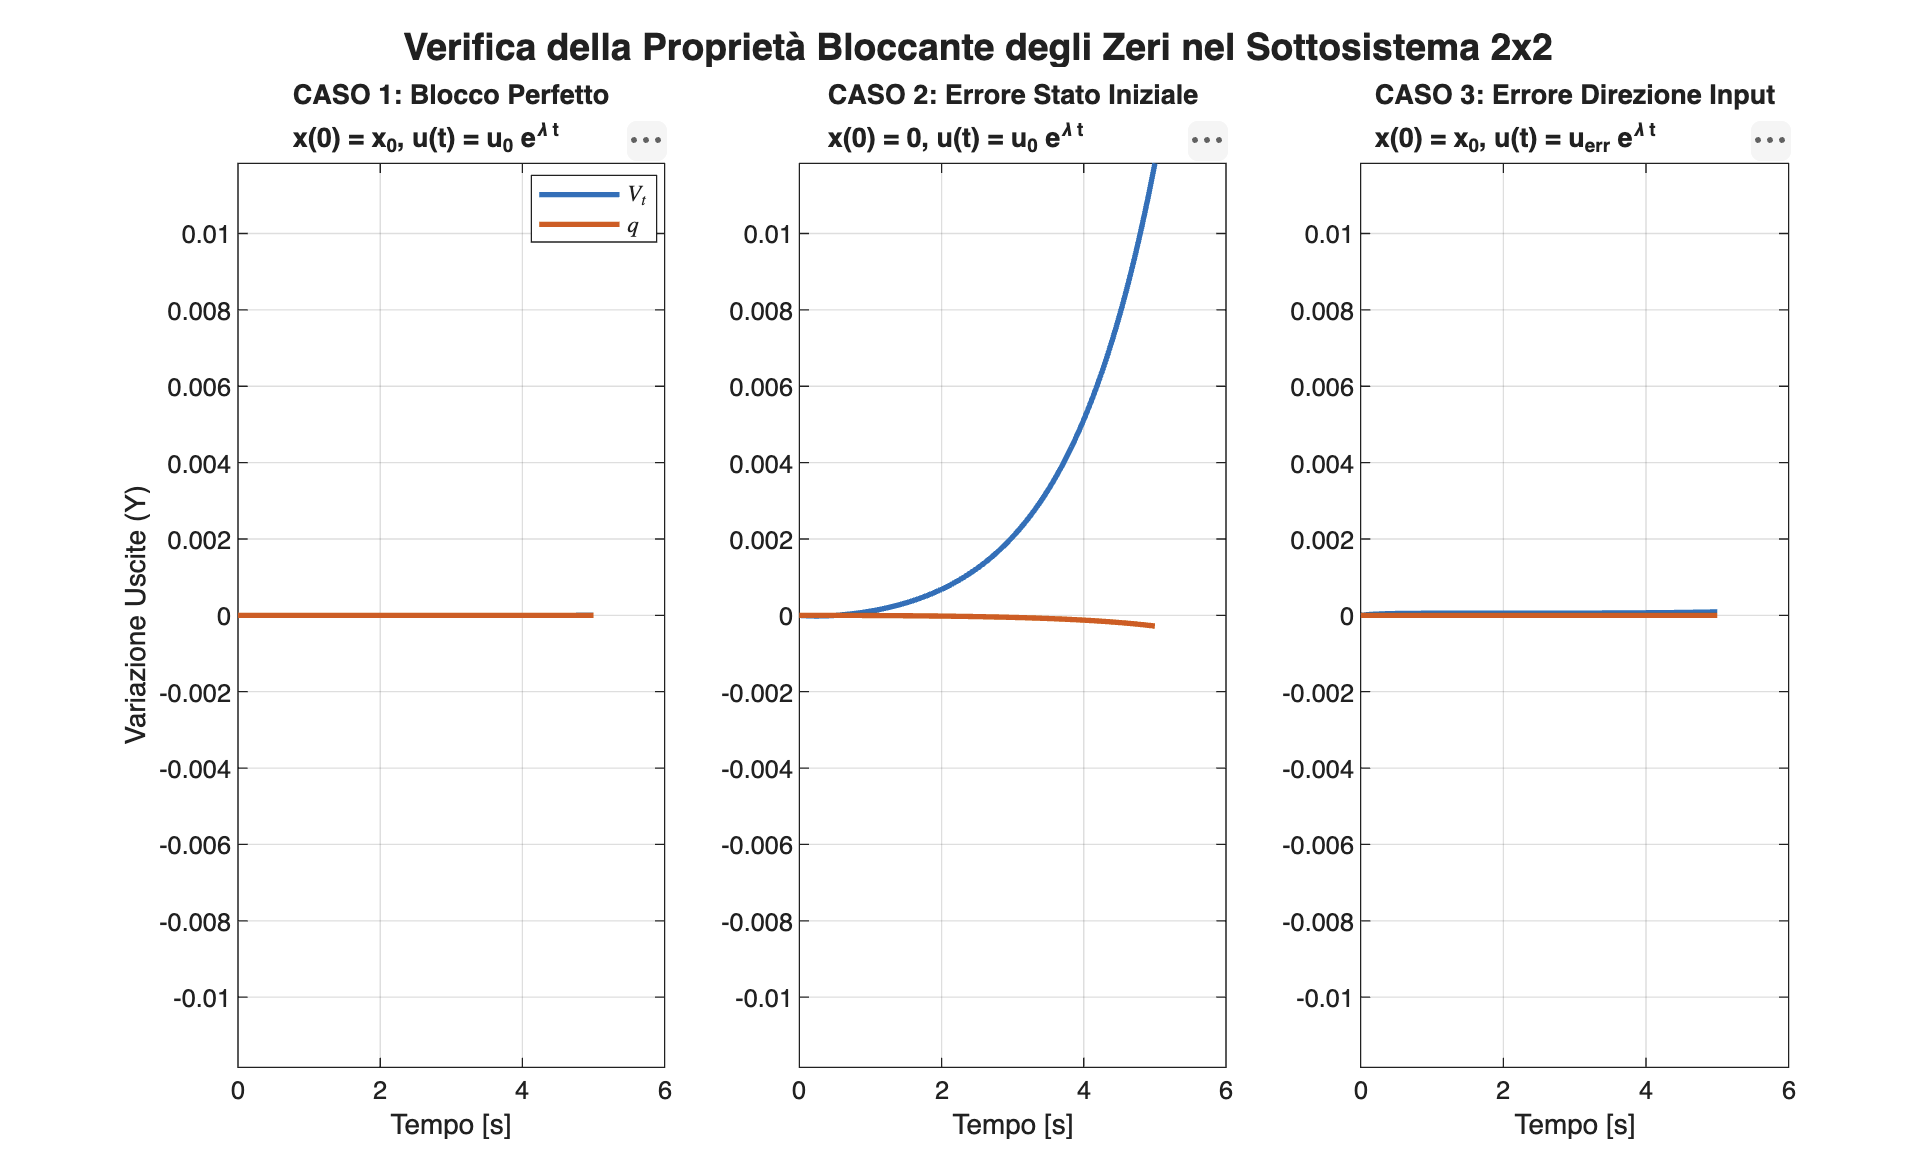
\includegraphics[width=1\linewidth]{Foto/blocantzero2x2_completa}
	\caption{Verifica simulata della proprietà bloccante sul sottosistema $2 \times 2$. Solo la perfetta sovrapposizione vettoriale tra ingresso e stato iniziale (Caso 1) garantisce l'annullamento delle uscite. Qualsiasi deviazione dallo stato geometrico ideale (Caso 2 e 3) compromette il bilanciamento delle forze interne.}
	\label{fig:blocantzero2x2_completa}
\end{figure}

\section{Interazioni dinamiche e vincoli strutturali}
L'esecuzione dell'algoritmo di linearizzazione e realizzazione minima sull'ambiente MATLAB ha prodotto la matrice $G_{min}(s)$ per il velivolo F-16 in condizione di trim. 

Un aspetto notevole della realizzazione minima è l'ordine del denominatore comune. Il polinomio caratteristico del sistema ridotto risulta essere di quarto grado:


\begin{equation}
	\Delta(s) = s^4 + 1.233 s^3 - 1.511 s^2 + 0.004179 s - 0.02174
\end{equation}
Questo denota che il sistema ha preservato tutte e quattro le variabili di stato essenziali della dinamica longitudinale ($\theta, q, U, W$). Inoltre, la presenza di variazioni di segno nei coefficienti del polinomio caratteristico conferma analiticamente, secondo il \textbf{criterio di stabilità di Routh-Hurwitz} \cite{ogata_2010}, l'intrinseca instabilità del velivolo discussa nel capitolo precedente.
Data la vastità della matrice completa (costituita da $5$ ingressi e $6$ uscite, per un totale di $30$ funzioni di trasferimento SISO) e considerando la natura sottoattuata del sistema, nei prossimi capitoli si procederà alla selezione di uno specifico sottoinsieme di ingressi e di uscite, definiti rispettivamente dalle matrici $B_{\text{ctrl}}$ e $C_{\text{ctrl}}$. Tale scelta risulta fondamentale per garantire l'effettivo controllo della dinamica longitudinale del velivolo, escludendo la componente dei disturbi atmosferici modellata nella matrice $B_{\text{wind}}$ (la cui trattazione estesa è rimandata al \hyperref[chap:disturbi_vento]{Cap.11}).